%---------------------------------------------------------------------
%
%                          Capítulo 5
%
%---------------------------------------------------------------------

\chapter{Text2LSE}


En este capítulo se muestra el desarrollo que se ha realizado a lo largo de este proyecto. Text2LSE es una aplicación web (ver Figura~\ref {fig: imgWebText2LSE}) que permite traducir textos escritos en castellano a LSE en formato vídeo y en formato imagen en tiempo real. Está basada en servicios web, los cuales están disponibles para todo el mundo de manera gratuita. Los vídeos e imágenes utilizados en la traducción a LSE son los recursos ofrecidos en el catálogo de LSE de ARASAAC. \\

En el apartado 5.1 se muestra la arquitectura de la aplicación web y cómo se comunica ésta con los servicios web. En el apartado 5.2 se explican en profundidad los servicios web desarrollados, tanto los utilizados en la aplicación web, como los desarrollados para aumentar las posibilidades de obtención de información para futuros desarrolladores. A continuación, en el apartado 5.3 se detalla más a fondo el desarrollo de la página web, tanto del diseño como de su funcionalidad. \\

La página web desarrollada es pública, y se puede acceder desde la siguiente url:

\begin{shaded}
	\url{https://holstein.fdi.ucm.es/tfg-text2lse }	
\end{shaded}

\begin{figure}[]
	\centering
	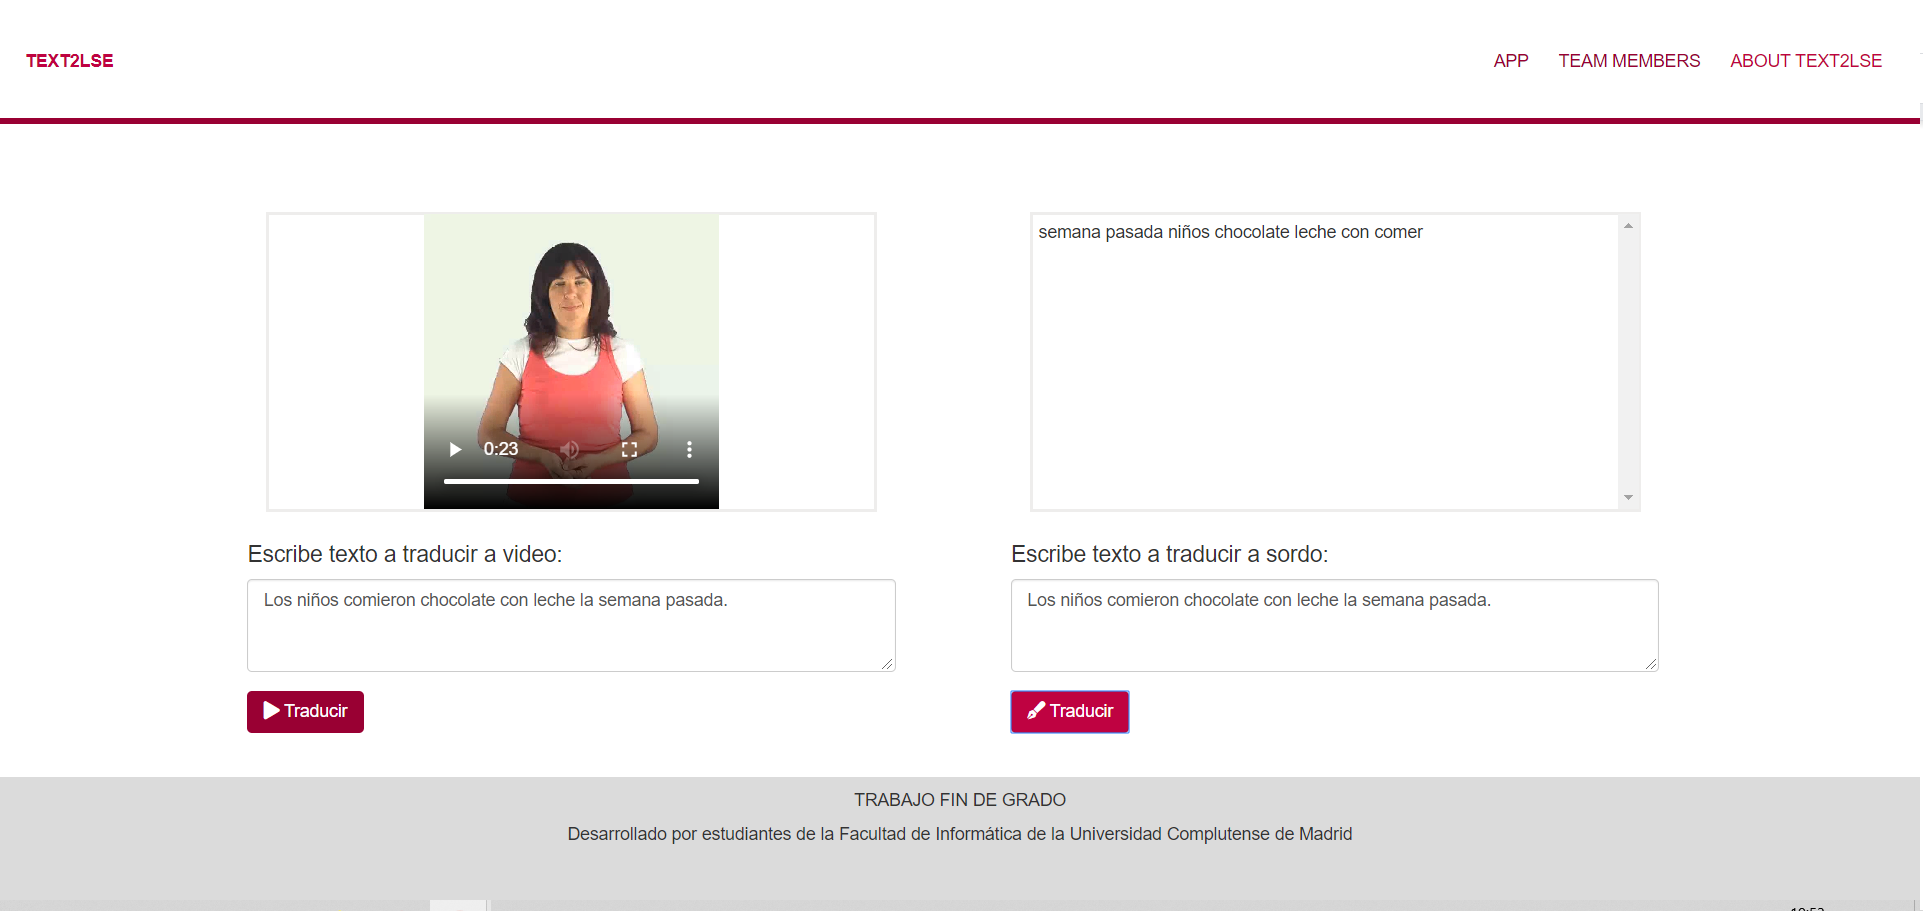
\includegraphics[width=1\textwidth]{Imagenes/Fuentes/Text2LSE/WebText2LSE.png}
	\caption{Aplicación web Text2LSE }
	\label {fig: imgWebText2LSE}
\end{figure}

%-------------------------------------------------------------------
\section{Arquitectura}
%-------------------------------------------------------------------
\label{cap4:sec:Arquitectura}

Text2LSE es una aplicación de traducción de castellano a LSE basada en servicios web, de manera que el código desarrollado sea fácilmente reutilizable. La arquitectura utilizada para el desarrollo de este proyecto es la arquitectura de cliente-servidor, es decir, un cliente muestra una web, la cual hace peticiones al servidor, que almacena los servicios web y devuelve la respuesta al cliente. Podemos ver un esquema de la arquitectura de este proyecto en la Figura~\ref {fig: imgArquitecturaText2LSE}.\\

Se ha optado por desarrollar una aplicación web debido a que ésta es accesible desde cualquier dispositivo que disponga de un navegador, ya sea un teléfono móvil, una tablet o un ordenador, sean de la marca y tamaño que sean. Para que se pueda ver de manera correcta en todos esos dispositivos, la aplicación web se ha desarrollado siguiendo un diseño responsive, es decir, que su visualización se adapte dependiendo de las dimensiones de la pantalla del dispositivo desde el cual se esté accediendo.\\

Respecto a la parte del servidor, se han desarrollado tres servicios web distintos, uno para devolver de manera rápida el vídeo en LSE de una sola palabra, otro para devolver el texto traducido a texto en LSE y otro para devolver el texto traducido a video en LSE. \\

Se ha utilizado un proxy inverso para poder acceder tanto a la página web como a los servicios web a través desde un mismo punto de acceso. Un Proxy inverso \citep*{proxyInverso} es un método de redireccionamiento del tráfico a partes específicas de una infraestructura concreta. Las principales finalidades para las que se usa este tipo de servidores son:

\begin{itemize}
	
	\item \textbf{Anonimización:} el proxy recibe todas las llamadas al servidor y se encarga de filtrarlas y redirigirlas como se haya configurado previamente. De esta manera, desde fuera del servidor no se va a poder obtener ningún tipo de información del servidor ni de los servicios que estén en él, solo se podrá obtener información del proxy.
	
	\item \textbf{Protección y cifrado:} al utilizar un proxy inverso se tiene la posibilidad de instalar sistemas de control y filtros de paquetes que protegen al servidor, aumentando así la seguridad del sistema.
	
	\item \textbf{Balanceo de carga:} permite redirigir las distintas solicitudes entrantes por varios servidores, permitiendo repartir la carga de trabajo para no sobrecargar ningún servidor o equilibrar la carga en el caso de que falle uno de ellos.
	
	\item \textbf{Caché:} el proxy se puede configurar para que sea capaz de almacenar las respuestas del servidor temporalmente para ofrecer una mayor velocidad de respuesta. De esta forma, si se recibe una solicitud cuya respuesta la tiene almacenada el proxy en su caché, se manda la respuesta de manera inmediata haciendo que no reciba tanta carga de procedimiento el back-end.
	
	\item \textbf{Compresión:} un proxy inverso también se puede utilizar como compresor de datos, tanto entrantes como salientes.
	
\end{itemize}

En este proyecto, se ha configurado el servidor Nginx como servidor proxy inverso con el fin de redirigir las distintas solicitudes al servidor correspondientes. Se han especificado una serie de rutas para diferenciar qué llamadas de usuario redireccionar a la página web y cuáles a los servicios web. Esta estructura se puede observar en la Figura~\ref {fig: imgProxy}.



\begin{figure}[]
	\centering
	
	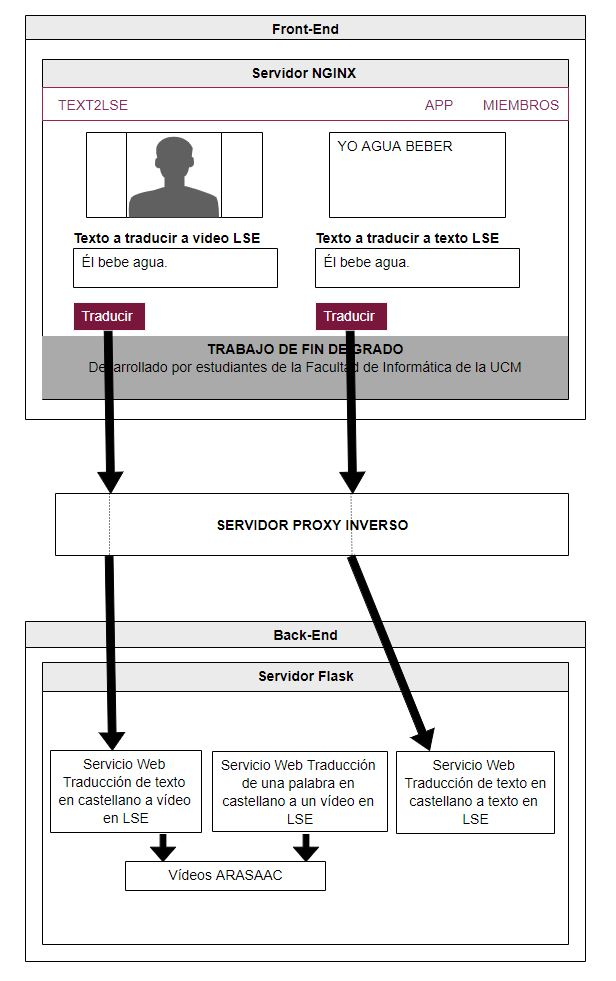
\includegraphics[width=1\textwidth]{Imagenes/Fuentes/Text2LSE/ArquitecturaText2LSE.jpg}
	\caption{Arquitectura de Text2LSE }
	\label {fig: imgArquitecturaText2LSE}
\end{figure}

\begin{figure}[]
	\centering
	
	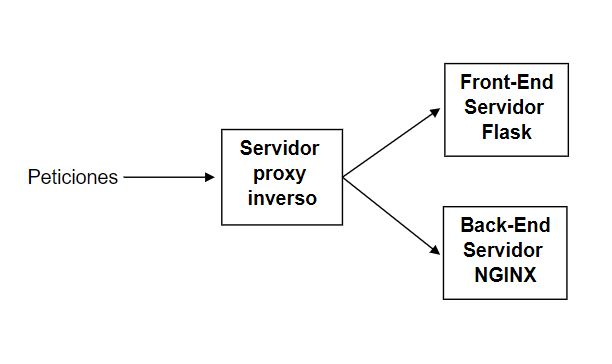
\includegraphics[width=1\textwidth]{Imagenes/Fuentes/Text2LSE/proxy.jpg}
	\caption{Esquema Proxy Inverso}
	\label {fig: imgProxy}
\end{figure}

\section{Back-End}

En esta sección se explican con detalle los servicios web desarrollados y su implementación. La API donde están implementados estos servicios es pública y en los siguientes apartados se indica la URL para acceder a cada servicio.

\begin{shaded}
	\url{https://holstein.fdi.ucm.es/tfg-text2lse }	
\end{shaded}



\subsection{Servicio web de traducción de palabra a LSE (vídeo)}

Este servicio permite obtener el video del signo en LSE correspondiente a una palabra determinada en lenguaje natural. Los videos utilizados en este servicio provienen del catálogo de vídeos de LSE de la web de ARASAAC. Para poder acceder a este servicio, se debe hacer una llamada GET a la API,  indicando la palabra que se desea traducir a LSE de la siguiente forma:\\

\begin{shaded}
	\url{https://holstein.fdi.ucm.es/tfg-text2lse/video/<palabra> }	
\end{shaded}

En el parámetro \textit{``palabra''} se debe indicar la palabra de la que se desea obtener su signo en LSE. \\

En caso de que se encuentre el vídeo de la palabra buscada, este servicio devuelve el vídeo deseado en formato mp4. En caso de que no se encuentre, devuelve un vídeo de error en formato .mp4. Este flujo lo podemos observar en la Figura~\ref {fig: imgFlujo1palabraText2LSE}. \\

Por ejemplo, para obtener el vídeo en LSE de la palabra \textit{``agua''}, como podemos ver en la Figura~\ref {fig: videoAgua}, se debe realizar la siguiente llamada:

\begin{shaded}
	\url{https://holstein.fdi.ucm.es/tfg-text2lse/video/agua }	
\end{shaded}


\begin{figure}[]
	\centering
	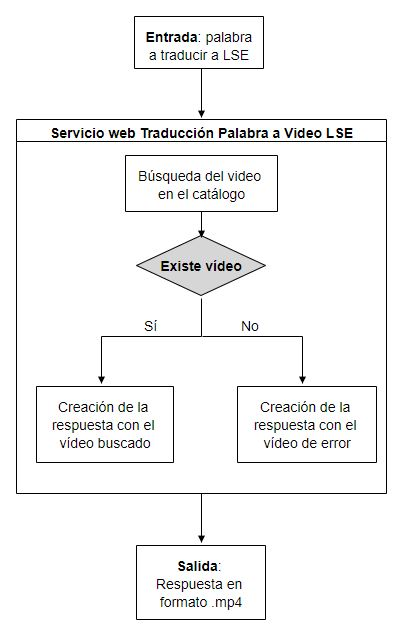
\includegraphics[width=0.7\textwidth]{Imagenes/Fuentes/Text2LSE/FlujoVideo1palabra.jpg}
	\caption{Flujo del servicio de Traducción de una palabra a vídeo en LSE}
	\label {fig: imgFlujo1palabraText2LSE}
\end{figure}

\begin{figure}[]
	\centering
	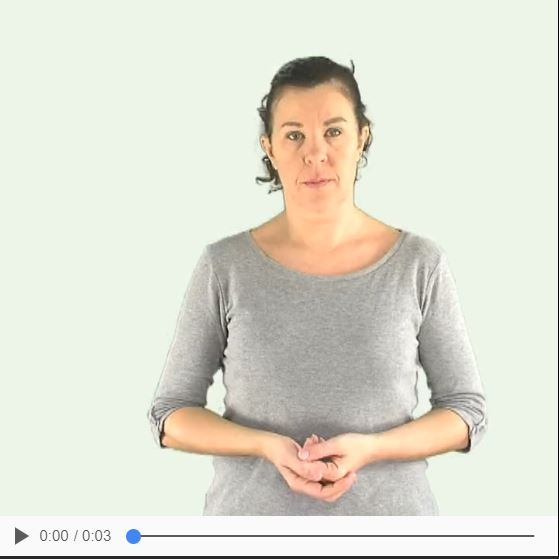
\includegraphics[width=0.5\textwidth]{Imagenes/Fuentes/Text2LSE/videoEjemplo.jpg}
	\caption{Vídeo devuelto por el servicio de traducción de la palabra \textit{``agua''} a LSE}
	\label {fig: videoAgua}
\end{figure}

\subsection{Servicio web de traducción de palabra a LSE (imagen)}

Este servicio permite obtener la imagen del signo en LSE correspondiente a una palabra determinada en lenguaje natural. Las imágenes utilizadas en este servicio provienen del catálogo de imágenes de LSE de la web de ARASAAC. Para poder acceder a este servicio, se debe hacer una llamada GET a la API,  indicando la palabra que se desea traducir a LSE de la siguiente forma:\\

\begin{shaded}
	\url{https://holstein.fdi.ucm.es/tfg-text2lse/imagen/<palabra> }	
\end{shaded}

En el parámetro \textit{``palabra''} se debe indicar la palabra de la que se desea obtener su signo en LSE. \\

En caso de que se encuentre la imagen de la palabra buscada, este servicio devuelve la imagen deseada .jpg. En caso de que no se encuentre, devuelve una imagen de error en formato .jpg. Este flujo lo podemos observar en la Figura~\ref {fig: imgFlujo1palabraImagenText2LSE}. \\

Por ejemplo, para obtener la imagen en LSE de la palabra \textit{``coche''}, como podemos ver en la Figura~\ref {fig: imgCoche}, se debe realizar la siguiente llamada:

\begin{shaded}
	\url{https://holstein.fdi.ucm.es/tfg-text2lse/imagen/coche }	
\end{shaded}


\begin{figure}[]
	\centering
	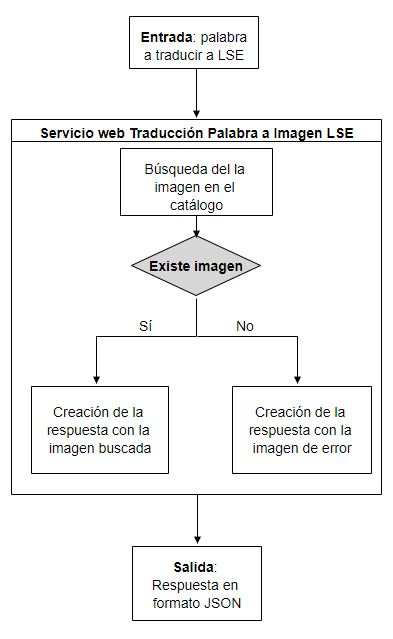
\includegraphics[width=0.7\textwidth]{Imagenes/Fuentes/Text2LSE/FlujoImagen1palabra.jpg}
	\caption{Flujo del servicio de Traducción de una palabra a imagen en LSE}
	\label {fig: imgFlujo1palabraImagenText2LSE}
\end{figure}

\begin{figure}[]
	\centering
	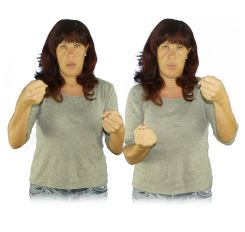
\includegraphics[width=0.5\textwidth]{Imagenes/Fuentes/Text2LSE/imagenEjemplo.jpg}
	\caption{Imagen devuelto por el servicio de traducción de la palabra \textit{``coche''} a LSE}
	\label {fig: imgCoche}
\end{figure}


\subsection{Servicio web para traducción de texto castellano a texto en LSE dependiendo de los vídeos existentes}

Este servicio implementa la funcionalidad de traducción de un texto en castellano a LSE en formato texto en función de los vídeos existentes en el sistema. Al igual que en el servicio anterior, los videos utilizados en este servicio provienen del catálogo de vídeos de LSE de la web de ARASAAC. Para poder acceder a este servicio, se debe realizar la siguiente petición POST a la API:\\

\begin{shaded}
	\url{https://holstein.fdi.ucm.es/tfg-text2lse/TextoLSEVideos/  }	
\end{shaded}


Los datos a enviar en la petición POST deben tener la siguiente estructura en JSON: 
\begin{center}
	
	\{ `Texto' : `<texto>' \}
	
\end{center}


En el parámetro \textit{``texto''} se debe incluir el texto que se desea traducir a LSE. Este flujo lo podemos observar en la Figura~\ref {fig: imgFlujoTextoVideoTextoText2LSE}.\\

Por ejemplo, para traducir el texto \textit{``Mis tías comen chocolate''} a LSE en formato texto en función de los vídeos existentes, se debe realizar la llamada POST indicada anteriormente con el siguiente JSON:


\begin{center}
	Entrada: \{ `Texto' : `Mis tías comen chocolate' \} \\
	Salida: \{ `Texto' : `yo tío mujer otro chocolate comer' \}
\end{center}

En este caso, al no encontrar el vídeo para la palabra \textit{``tías''} busca el vídeo de esa palabra sin morfemas de género y número, en este caso busca el vídeo de la palabra \textit{``tío''} añadiendo la palabra  \textit{``mujer''} para indicar el femenino y la palabra  \textit{``otro''} para indicar el plural.


\begin{figure}[]
	\centering
	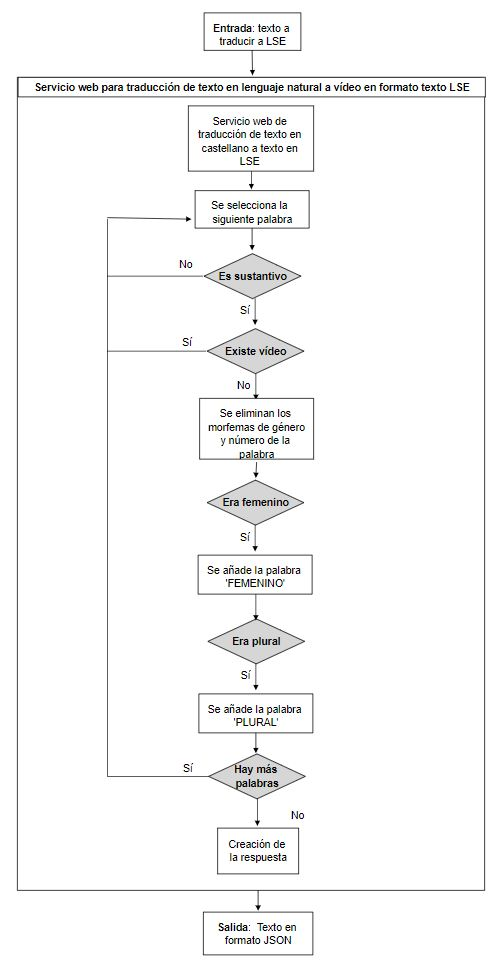
\includegraphics[width=0.8\textwidth]{Imagenes/Fuentes/Text2LSE/FlujoTextoVideoTexto.jpg}
	\caption{ Flujo servicio de traducción de texto en castellano a texto en LSE en función de los vídeos existentes }
	\label {fig: imgFlujoTextoVideoTextoText2LSE}
\end{figure}

\subsection{Servicio web para traducción de texto castellano a texto en LSE dependiendo de las imágenes existentes}

Este servicio implementa la funcionalidad de traducción de un texto en castellano a LSE en formato texto en función de las imágenes existentes en el sistema. Al igual que en el servicio anterior, las imágenes utilizados en este servicio provienen del catálogo de imágenes de LSE de la web de ARASAAC. Para poder acceder a este servicio, se debe realizar la siguiente petición POST a la API:\\

\begin{shaded}
	\url{https://holstein.fdi.ucm.es/tfg-text2lse/textoImagen/  }	
\end{shaded}


Los datos a enviar en la petición POST deben tener la siguiente estructura en JSON: 
\begin{center}
	
	\{ `Texto' : `<texto>' \}
	
\end{center}


En el parámetro \textit{``texto''} se debe incluir el texto que se desea traducir a LSE. Este flujo lo podemos observar en la Figura~\ref {fig: imgFlujoTextoImagenTextoText2LSE}.\\

Por ejemplo, para traducir el texto \textit{``Los caballos son rápidos''} a LSE en formato texto en función de los vídeos existentes, se debe realizar la llamada POST indicada anteriormente con el siguiente JSON:


\begin{center}
	Entrada: \{ `Texto' : `Los caballos son rápidos' \} \\
	Salida: \{ `Texto' : `caballo otro rápido' \}
\end{center}

En este caso, al no encontrar la imagen para la palabra \textit{``caballos''} busca el vídeo de esa palabra sin morfemas de género y número, en este caso busca el vídeo de la palabra \textit{``caballo''} añadiendo la palabra  \textit{``otro''} para indicar el plural.


\begin{figure}[]
	\centering
	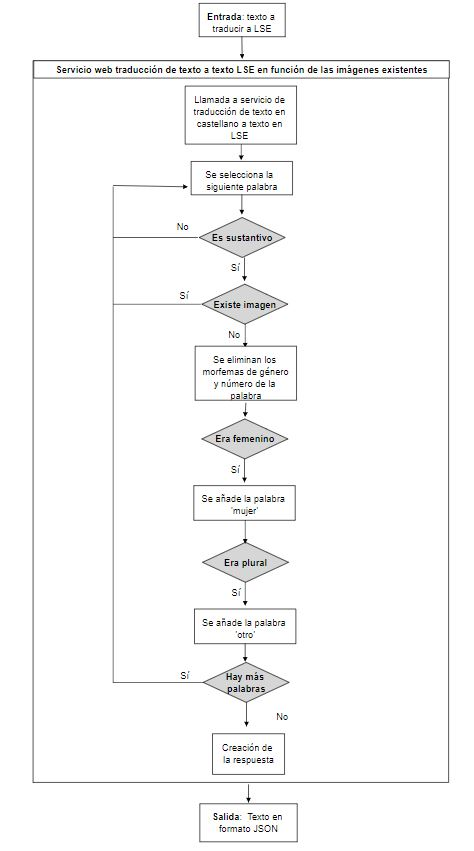
\includegraphics[width=0.8\textwidth]{Imagenes/Fuentes/Text2LSE/FlujoTextoImagenTexto.jpg}
	\caption{ Flujo servicio de traducción de texto en castellano a texto en LSE en función de las imágenes existentes }
	\label {fig: imgFlujoTextoImagenTextoText2LSE}
\end{figure}


\subsection{Servicio web para traducción de texto a LSE (vídeo)}

Este servicio implementa la funcionalidad de traducción de un texto en castellano a LSE en formato video. Al igual que en el servicio anterior, los videos utilizados en este servicio provienen del catálogo de vídeos de LSE de la web de ARASAAC. Para poder acceder a este servicio, se debe realizar la siguiente petición POST a la API:\\

\begin{shaded}
	\url{https://holstein.fdi.ucm.es/tfg-text2lse/video/  }	
\end{shaded}


Los datos a enviar en la petición POST deben tener la siguiente estructura en JSON: 
\begin{center}

		\{ 'Texto' : '<texto>' \}

\end{center}


En el parámetro \textit{``texto''} se debe incluir el texto que se desea traducir a LSE. En caso de que se encuentren los recursos para traducir las palabras solicitadas en formato vídeo, se ejecuta un proceso que junta todos los vídeos en uno solo. Este vídeo es el que devuelve el servicio en formato mp4. Este flujo lo podemos observar en la Figura~\ref {fig: imgFlujoVideoTextoText2LSE}.\\

Por ejemplo, para obtener el vídeo en LSE del texto \textit{``Los niños comen chocolate''}, como podemos ver en la Figura~\ref {fig: videoOracion}, se debe realizar la llamada POST indicada anteriormente con el siguiente JSON:

\begin{center}
	
	\{ `Texto' : `Los niños comen chocolate' \}
	
\end{center}


\begin{figure}[]
	\centering
	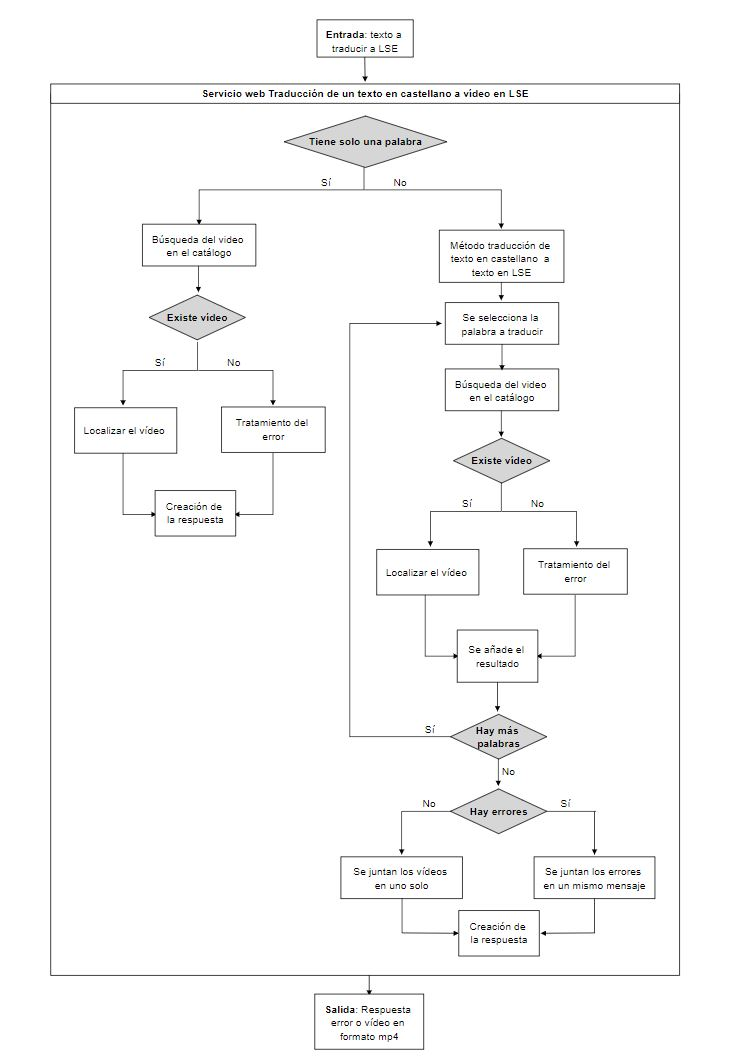
\includegraphics[width=1\textwidth]{Imagenes/Fuentes/Text2LSE/FlujoVideoTexto.jpg}
	\caption{ Flujo servicio de traducción de texto en castellano a LSE en formato vídeo }
	\label {fig: imgFlujoVideoTextoText2LSE}
\end{figure}

\begin{figure}[]
	\centering
	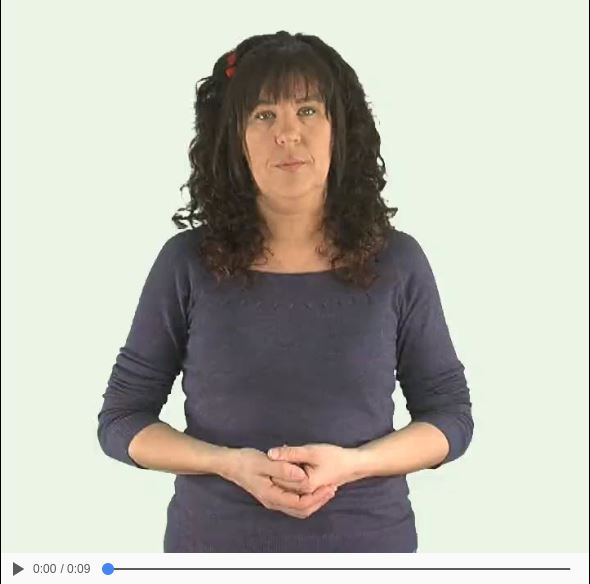
\includegraphics[width=0.5\textwidth]{Imagenes/Fuentes/Text2LSE/videoOracion.jpg}
	\caption{Vídeo devuelto por el servicio de traducción del texto \textit{``Los niños comen chocolate''} a LSE}
	\label {fig: videoOracion}
\end{figure}

\subsubsection{Servicio web para Traducción de texto en castellano a texto en LSE}
Este servicio implementa la funcionalidad de traducción de un texto en castellano a LSE en formato texto.
Para poder acceder a este servicio, se debe realizar una petición POST a la API en la siguiente URL:


\subsection{Servicio web para Traducción de texto en castellano a texto en LSE}
Este servicio implementa la funcionalidad de traducción de un texto en castellano a LSE en formato texto.
Para poder acceder a este servicio, se debe realizar una petición POST a la API en la siguiente URL:


\begin{shaded}
	\url{https://holstein.fdi.ucm.es/tfg-text2lse/TextoLSE}	
\end{shaded}


Los datos a enviar en la petición POST deben tener la siguiente estructura en JSON: 
\begin{center}
	
	\{ 'Texto' : '<texto>' \}
	
\end{center}


En el parámetro `texto' se debe incluir el texto que se desea traducir a LSE. Un ejemplo de uso sería: 
 

En el parámetro `texto' se debe incluir el texto que se desea traducir a LSE. Un ejemplo de uso sería: 




\begin{center}

 Entrada:  \{ 'Texto' : 'El niño bebe agua.' \}\\
 Salida:   \{ 'Texto' : 'niño agua beber.' \}

	Entrada:  \{ 'Texto' : 'El niño bebe agua.' \}\\
	Salida:   \{ 'Texto' : 'niño agua beber.' \}

\end{center}


El flujo de este servicio web lo podremos ver en la Figura~\ref {fig: imgFlujoFlujoTextoLSE}.


\begin{figure}[]
	\centering
	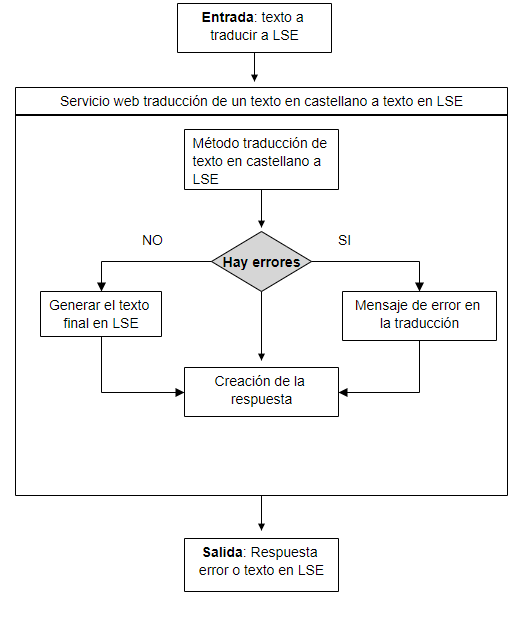
\includegraphics[width=1\textwidth]{Imagenes/Fuentes/Text2LSE/FlujoTextoLSE.png}
	\caption{ Flujo servicio de traducción de texto en castellano a texto en LSE }
	\label {fig: imgFlujoFlujoTextoLSE}
\end{figure}

Para que el servicio web sea capaz de traducir una frase a la LSE se ha tenido que realizar un procesamiento previo del texto en castellano para poder adaptarlo a la Lengua de Signos Española. A pesar de disponer herramientas PLN de la Universidad, debido a la singularidad de Lengua de Signos y a la falta de tiempo para aprender a usa una herramienta nueva debido a su complejidad el procesamiento del Lenguaje Natural ha sido implementado desde cero por los tres integrantes del equipo utilizando únicamente la herramienta Spacy. \\


La implementación del PLN está basada en un sistema de reglas las cuales filtran qué palabras deben de ser utilizadas y cuales no. La elección a la hora de desarrollar el Procesamiento del Lenguaje Natural para nuestro proyecto estaba entre un sistema basado en reglas o mediante el uso de aprendizaje automático. La opción de desarrollar un aprendizaje automático no era viable debido a la dificultad y la falta de ejemplos en castellano para entrenar el sistema. Por este motivo se eligió el sistema basado en reglas ya que era más fácil de implementar y aunque puede limitar la capacidad de traducción de frases que no cumplan dichas reglas, cumple con los objetivos marcados en el proyecto que es traducir frases simples a LSE.\\

Nuestro PLN se divide en tres fases.Lo primero que hace es recopilar información de la frase en castellano para luego realizar un análisis sintáctico y morfológico de la frase y así poder ordenarla respetando la estructura de la LSE. A continuación se explicará con más detalle cada una de las fases:

\subsubsection{Recopilar la  información} 
Para poder realizar los análisis sintácticos y morfológicos de la frase se necesita obtener toda la información posible de la frase. Para ello se realizará el proceso de Tokenización el cual divide la frase en una lista de palabras las cuales pasan a denominarse \textit{tokens} pero con la diferencia de que ahora cada token contiene gran cantidad de información. Esta información es:


\begin{itemize}
	
	\item \textbf{Dependencia:} función de la palabra dentro de la frase. Ejemplo: `
	\item \textbf{Tags:} información de la palabra como el género, el número, el tiempo verbal, etc.
	\item \textbf{Part of speech:} tipo de palabra como nombre, adjetivo, etc.
	\item \textbf{Lema:} Lema de palabra.	
	
\end{itemize}


Por ejemplo la información que se obtendría del la oración \textit{`Los niños merendaron chocolate'} sería ~\ref {fig: tokenInformacion}:
\begin{figure}[h]
	\centering
	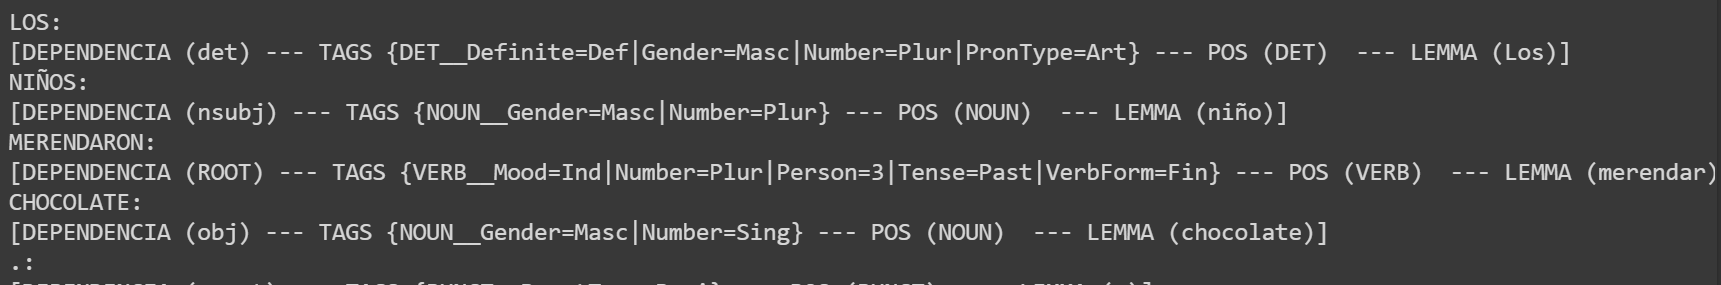
\includegraphics[width=1 \textwidth]{Imagenes/Fuentes/PNL/InfoPLN.png}
	\caption{ Información de la frase Los niños merendaron chocolate}
	\label {fig: tokenInformacion}
\end{figure}



\subsubsection{Análisis sintáctico} 
Una vez separado la oración en tokens hay que diferenciar que palabras forman parte del sujeto y cuales del predicado. Para ello hay que recorrer el árbol de dependencias mediante una función recursiva empezando desde el ROOT que es el token raíz del cual dependen todos los demás. Para entender cómo funcionan las dependencias se va a utilizar como ejemplo la oración `Ayer los niños merendaban chocolate'. En la Figura ~\ref {fig: dependencias} se muestran las dependencias de esta frase.

\begin{figure}[h]
	\centering
	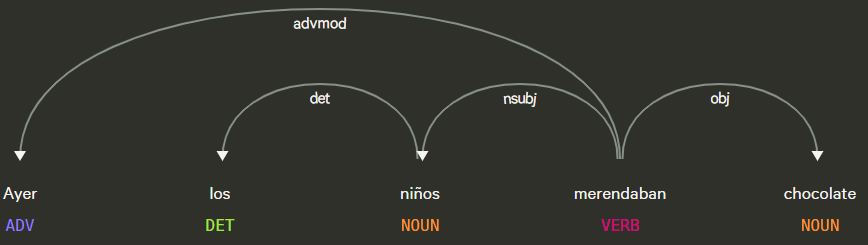
\includegraphics[width=1\textwidth]{Imagenes/Fuentes/Text2LSE/dependencias.png}
	\caption{ Displacy grafo de dependencias }
	\label {fig: dependencias}
\end{figure}


Como se puede apreciar en el diagrama del token `merendaban' dependen tres tokens (Ayer, niños y chocolate) y de ellos también dependen otros y así sucesivamente. Estas dependencias se traducen en un árbol donde el ROOT es la raíz como podemos ver en la Figura~\ref {fig: grafo}:\\


\begin{figure}[]
	\centering
	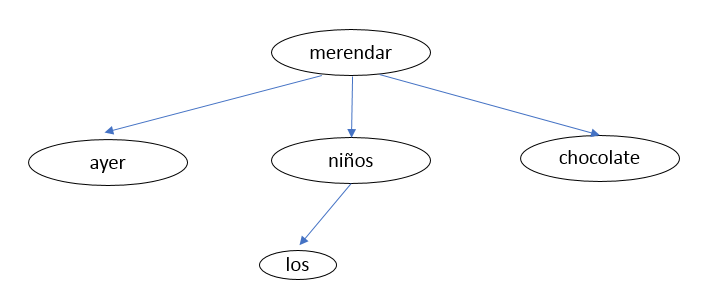
\includegraphics[width=1\textwidth]{Imagenes/Fuentes/Text2LSE/grafo.png}
	\caption{ Árbol generado para la frase Los niños merendaron chocolate }
	\label {fig: grafo}
\end{figure}


Para obtener las distintas partes de la oración se recorre el árbol de la siguiente forma. Lo primero es obtener el sujeto y para ello hay que buscar el token que contenga la dependencia ``nsuj''. Una vez encontrado hay que volver a llamar a la función recursiva para obtener los hijos y guardarlos en una lista. En el ejemplo anterior \textit{``Ayer los niños merendaban chocolate''} el sujeto sería (Los niños). Una vez obtenido los tokens que pertenecen al sujeto, los tokens restantantes pertenecen al predicado (Ayer, merendaban y chocolate) y añaden a una lista.
\begin{center}
	\begin{itemize}
		\item \textbf{Sujeto:}  [Los, niños]
		\item \textbf{Predicado:} [Ayer, merendaban, chocolate]
		
	\end{itemize}
\end{center}
\subsubsection{Análisis morfológico} 

La Lengua de Signos Española tiene una estructura gramatical diferente al castellano y como el objetivo del TFG es llegar a traducir frases simples a LSE, la estructura de la oración que se ha tomado como referencia siguiente:
\begin{center}
	TIEMPO + SUJETO + OBJETO + VERBO.
\end{center}

A parte de seguir esta estructura, en la LSE las palabras pueden tener un orden distinto al castellano o se pueden añadir o eliminar palabras que la oración original en castellano no estaban.

El análisis morfológico que hemos seguido es a la hora de añadir o quitar palabras de la oración para poder obtener una traducción lo mas real posible es el siguiente:

\begin{itemize}
	
	\item \textbf{Determinantes:} Los determinantes se omiten a la hora de hacer la traducción. \textit{Ejemplo: ``El niño come carne''} se traduce como \textit{``Niño carne comer''.}
	\item \textbf{Verbos copulativos:} Los verbos copulativos ser, estar o parecer se omiten a la hora de la traducción. \textit{Ejemplo: ``yo soy bajo''} se traduce como \textit{``yo bajo''.}
	
	\item \textbf{Posesivos:} Los determinantes posesivos se sustituyen por pronombres personales.  \textit{Ejemplo: ``Mi niño es bajo''} se traduce como \textit{``yo niño bajo''.}
	
	\item \textbf{Preposiciones:} Algunas preposiciones se quitan y otras se añaden.  \textit{Ejemplo: ``Mi niño está en el parque''} se traduce como \textit{``yo hijo parque''.}
	
	\item \textbf{Adjetivos:} Los adjetivos se ponen en masculino.  \textit{Ejemplo: ``Mi mamá es fea''} se traduce como \textit{``yo mamá feo''.}
	

	\item \textbf{Temporalidad:} La temporalidad como vemos en la estructura de más arriba va al principio de la oración. \textit{Ejemplo: ``Yo comí chocolate ayer''} se traduce como \textit{``Ayer yo chocolate comer''.} Sin embargo no siempre hay adverbios de tiempo en la oración que indican la temporalidad. Quién indica en este caso el tiempo es el verbo por lo que habría que añadir la temporalidad con las signos PASADO o FUTURO.
	\textit{Ejemplo: ``Yo comeré chocolate''} se traduce como \textit{``Futuro yo chocolate comer''.}
		

	\item \textbf{Temporalidad:} La temporalidad como vemos en la estructura de más arriba va al principio de la oración. \textit{Ejemplo: ``Yo comí chocolate ayer''} se traduce como \textit{``Ayer yo chocolate comer''.} Sin embargo no siempre hay adverbios de tiempo en la oración que indican la temporalidad. Quién indica en este caso el tiempo es el verbo por lo que habría que añadir la temporalidad con las signos PASADO o FUTURO.
	\textit{Ejemplo: ``Yo comeré chocolate''} se traduce como \textit{``Futuro yo chocolate comer''.}
	

\end{itemize}


Una vez añadido y quitado las palabras el sujeto y predicado, la frase se tiene que ordenar según la estructura tiempo + sujeto + objeto + verbo por lo que el resultado final de la frase usada como ejemplo ``Los niños ayer merendaban chocolate'' sería: 

\begin{center}
	\begin{itemize}
		\item \textbf{Sujeto:}  [niños]
		\item \textbf{Predicado:} [Ayer, merendar, chocolate]
		\item \textbf{Frase ordenada:} ``Ayer niños chocolate merendar'' 
		
		
	\end{itemize}
\end{center}


\subsection{Servicio web para traducción de texto castellano a texto en LSE dependiendo de los vídeos existentes}

Este servicio implementa la funcionalidad de traducción de un texto en castellano a LSE en formato texto en función de los vídeos existentes en el sistema. Al igual que en el servicio anterior, los videos utilizados en este servicio provienen del catálogo de vídeos de LSE de la web de ARASAAC. Para poder acceder a este servicio, se debe realizar la siguiente petición POST a la API:\\

\begin{shaded}
	\url{https://holstein.fdi.ucm.es/tfg-text2lse/TextoLSEVideos/  }	
\end{shaded}


Los datos a enviar en la petición POST deben tener la siguiente estructura en JSON: 
\begin{center}
	
	\{ `Texto' : `<texto>' \}
	
\end{center}


En el parámetro \textit{``texto''} se debe incluir el texto que se desea traducir a LSE. Este flujo lo podemos observar en la Figura~\ref {fig: imgFlujoTextoVideoTextoText2LSE}.\\

Por ejemplo, para traducir el texto \textit{``Mis tías comen chocolate''} a LSE en formato texto en función de los vídeos existentes, se debe realizar la llamada POST indicada anteriormente con el siguiente JSON:


\begin{center}
	Entrada: \{ `Texto' : `Mis tías comen chocolate' \} \\
	Salida: \{ `Texto' : `yo tío mujer otro chocolate comer' \}
\end{center}

En este caso, al no encontrar el vídeo para la palabra \textit{``tías''} busca el vídeo de esa palabra sin morfemas de género y número, en este caso busca el vídeo de la palabra \textit{``tío''} añadiendo la palabra  \textit{``mujer''} para indicar el femenino y la palabra  \textit{``otro''} para indicar el plural.


\begin{figure}[]
	\centering
	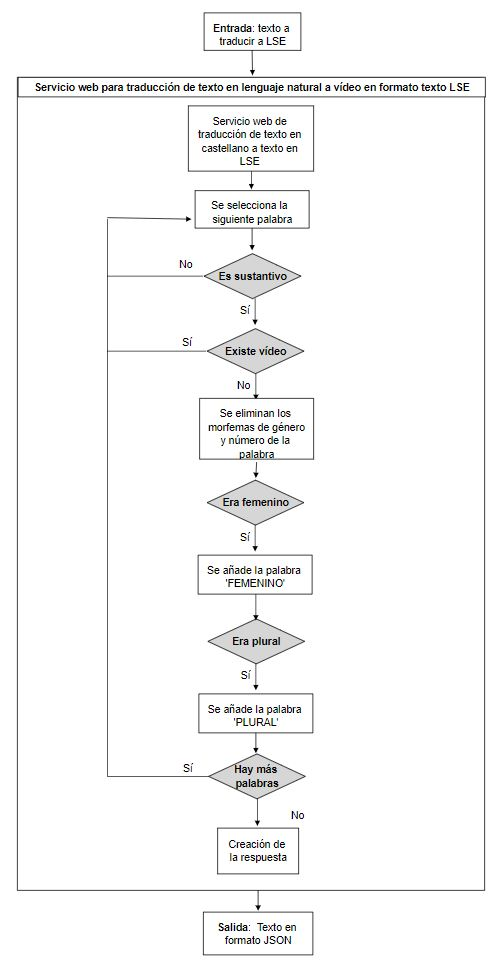
\includegraphics[width=0.8\textwidth]{Imagenes/Fuentes/Text2LSE/FlujoTextoVideoTexto.jpg}
	\caption{ Flujo servicio de traducción de texto en castellano a texto en LSE en función de los vídeos existentes }
	\label {fig: imgFlujoTextoVideoTextoText2LSE}
\end{figure}

\subsection{Servicio web para traducción de texto castellano a texto en LSE dependiendo de las imágenes existentes}

Este servicio implementa la funcionalidad de traducción de un texto en castellano a LSE en formato texto en función de las imágenes existentes en el sistema. Al igual que en el servicio anterior, las imágenes utilizados en este servicio provienen del catálogo de imágenes de LSE de la web de ARASAAC. Para poder acceder a este servicio, se debe realizar la siguiente petición POST a la API:\\

\begin{shaded}
	\url{https://holstein.fdi.ucm.es/tfg-text2lse/textoImagen/  }	
\end{shaded}


Los datos a enviar en la petición POST deben tener la siguiente estructura en JSON: 
\begin{center}
	
	\{ `Texto' : `<texto>' \}
	
\end{center}


En el parámetro \textit{``texto''} se debe incluir el texto que se desea traducir a LSE. Este flujo lo podemos observar en la Figura~\ref {fig: imgFlujoTextoImagenTextoText2LSE}.\\

Por ejemplo, para traducir el texto \textit{``Los caballos son rápidos''} a LSE en formato texto en función de los vídeos existentes, se debe realizar la llamada POST indicada anteriormente con el siguiente JSON:


\begin{center}
	Entrada: \{ `Texto' : `Los caballos son rápidos' \} \\
	Salida: \{ `Texto' : `caballo otro rápido' \}
\end{center}

En este caso, al no encontrar la imagen para la palabra \textit{``caballos''} busca el vídeo de esa palabra sin morfemas de género y número, en este caso busca el vídeo de la palabra \textit{``caballo''} añadiendo la palabra  \textit{``otro''} para indicar el plural.


\begin{figure}[]
	\centering
	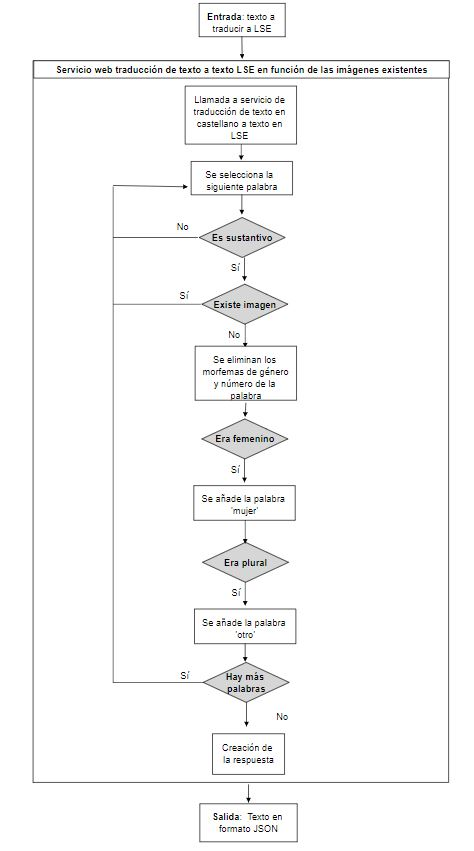
\includegraphics[width=0.8\textwidth]{Imagenes/Fuentes/Text2LSE/FlujoTextoImagenTexto.jpg}
	\caption{ Flujo servicio de traducción de texto en castellano a texto en LSE en función de las imágenes existentes }
	\label {fig: imgFlujoTextoImagenTextoText2LSE}
\end{figure}


\subsection{Servicio web para traducción de texto a LSE (vídeo)}

Este servicio implementa la funcionalidad de traducción de un texto en castellano a LSE en formato video. Al igual que en el servicio anterior, los videos utilizados en este servicio provienen del catálogo de vídeos de LSE de la web de ARASAAC. Para poder acceder a este servicio, se debe realizar la siguiente petición POST a la API:\\

\begin{shaded}
	\url{https://holstein.fdi.ucm.es/tfg-text2lse/video/  }	
\end{shaded}


Los datos a enviar en la petición POST deben tener la siguiente estructura en JSON: 
\begin{center}

		\{ 'Texto' : '<texto>' \}

\end{center}


En el parámetro \textit{``texto''} se debe incluir el texto que se desea traducir a LSE. En caso de que se encuentren los recursos para traducir las palabras solicitadas en formato vídeo, se ejecuta un proceso que junta todos los vídeos en uno solo. Este vídeo es el que devuelve el servicio en formato mp4. Este flujo lo podemos observar en la Figura~\ref {fig: imgFlujoVideoTextoText2LSE}.\\

Por ejemplo, para obtener el vídeo en LSE del texto \textit{``Los niños comen chocolate''}, como podemos ver en la Figura~\ref {fig: videoOracion}, se debe realizar la llamada POST indicada anteriormente con el siguiente JSON:

\begin{center}
	
	\{ `Texto' : `Los niños comen chocolate' \}
	
\end{center}


\begin{figure}[]
	\centering
	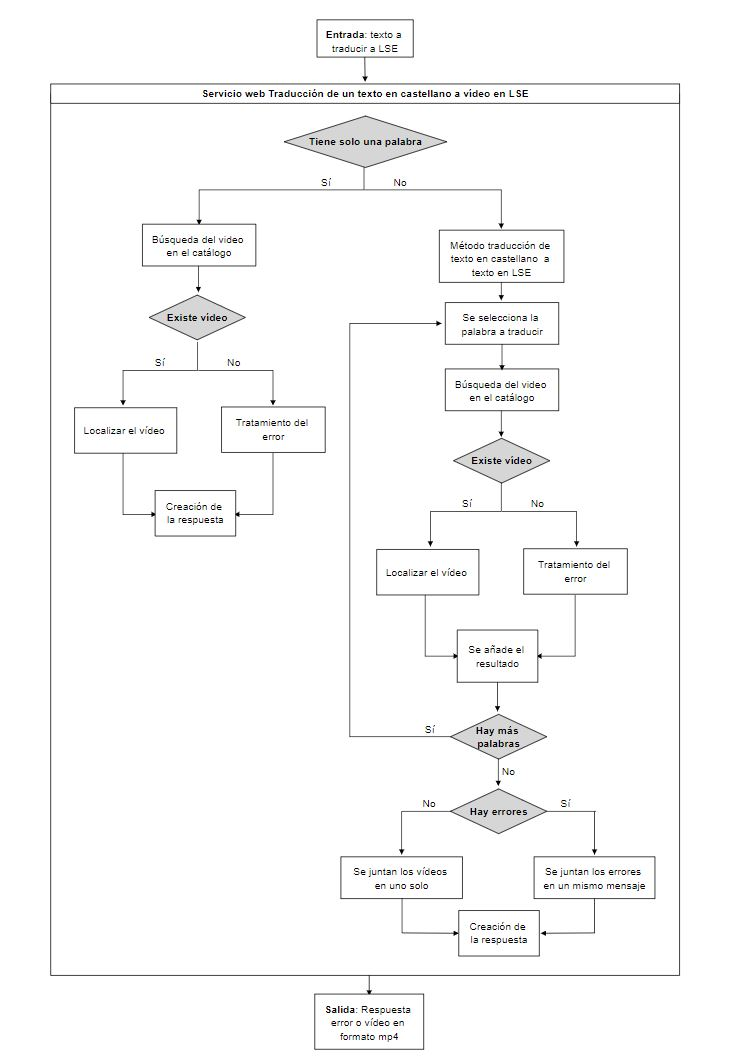
\includegraphics[width=1\textwidth]{Imagenes/Fuentes/Text2LSE/FlujoVideoTexto.jpg}
	\caption{ Flujo servicio de traducción de texto en castellano a LSE en formato vídeo }
	\label {fig: imgFlujoVideoTextoText2LSE}
\end{figure}

\begin{figure}[]
	\centering
	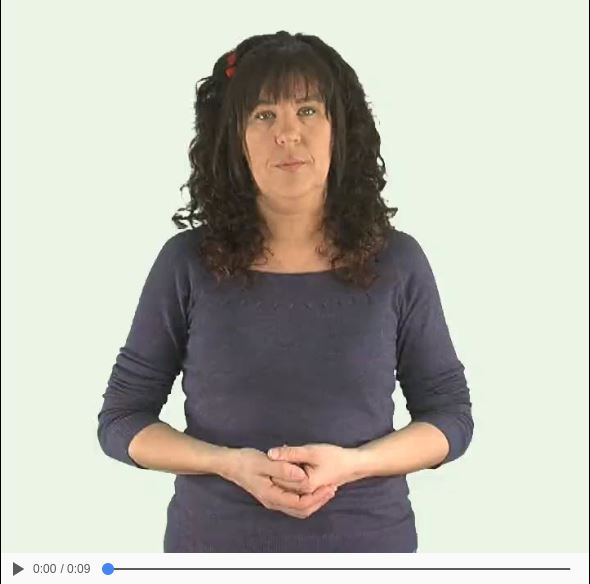
\includegraphics[width=0.5\textwidth]{Imagenes/Fuentes/Text2LSE/videoOracion.jpg}
	\caption{Vídeo devuelto por el servicio de traducción del texto \textit{``Los niños comen chocolate''} a LSE}
	\label {fig: videoOracion}
\end{figure}




\section{Front-End}

En esta sección se explica en detalle la aplicación web desarrollada, cuya finalidad es proporcionar a los usuarios una interfaz sencilla donde puedan introducir el texto que desean traducir y obtener la traducción del texto en LSE, tanto en imágenes como en vídeo. En la  Figura~\ref {fig: imgWebText2LSE} se muestra la interfaz de la aplicación, que consta de un input donde el usuario podrá introducir el texto en castellano que desee traducir, un desplegable donde podrá seleccionar el formato de salida y un botón para realizar la traducción.\\

Los formatos de salida disponibles en el desplegable son los siguientes:

\begin{itemize}

	\item \textbf{Traducción a vídeo:} tras seleccionar este formato y pulsar el botón ``traducir'', se realizará una llamada Fetch al microservicio de traducción a Texto Castellano a texto LSE dependiendo de los videos existentes, pasando por el servidor proxy, que a su vez redirigirá la petición a la API. Una función Fetch se encargará de recibir el texto resultante y de llamar por cada una de esas palabras al servicio que devuelve el video LSE correspondiente. Posteriormente se incrustan todos los vídeos en orden en el código HTML, de tal manera que se reproduce uno detrás de otro. Así, se podrá visualizar por pantalla un vídeo en el que se podrá ver a un intérprete de ARASAAC realizando los signos LSE correspondientes.
	
	\item \textbf{Traducción a imágenes:} de la misma manera que en el caso de los vídeos, tras seleccionar este formato y pulsar el botón ``traducir'', se realizará una llamada Fetch  al microservicio de traducción a Texto Castellano a texto LSE dependiendo de las imágenes existentes, pasando por el servidor proxy, que a su vez redirigirá la petición a la API. Una función Fetch se encargará de recibir el texto resultante y de llamar por cada una de esas palabras al servicio que devuelve la imagen LSE correspondiente. Posteriormente se incrustan todas las imágenes en orden en el código HTML. 

	\item \textbf{Traducción a texto LSE:} tras seleccionar este formato y pulsar el botón ``traducir'' se llamará a una función Fetch que realizará una petición a la url correspondiente. En caso de éxito aparecerá por pantalla dicho texto traducido a texto LSE.

\end{itemize}


En caso de error en cualquiera de las dos funcionalidades, la aplicación mostrará un modal con el tipo y detalle del error obtenido al realizar la petición a la API donde se encuentran nuestros servicios web.\\ 

Por otro lado, la interfaz también cuenta con un menú en la parte superior, donde además de a la página principal podemos acceder a una página con información sobre los miembros del equipo y de los tutores, y a otra con información sobre la aplicación. Todo ello se ha implementado siguiendo un diseño responsive, haciendo uso de Bootstrap 3, para garantizar que la herramienta sea accesible desde cualquier dispositivo. En la Figura~\ref {fig: imgResponsive} podemos observar la interfaz vista desde un dispositivo móvil.\\


\begin{figure}[]
	\centering
	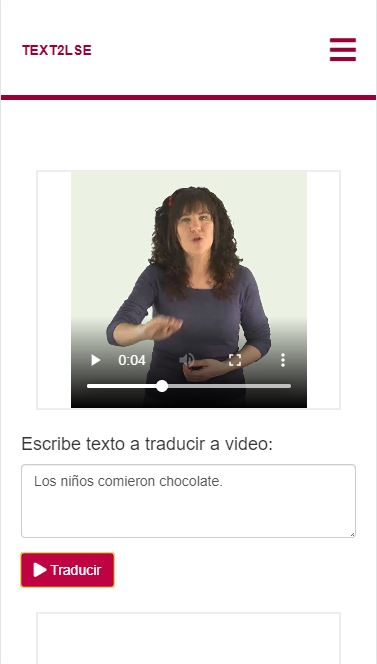
\includegraphics[width=0.75\textwidth]{Imagenes/Fuentes/Text2LSE/responsive.jpg}
	\caption{ Aplicación Web vista desde un dispositivo móvil }
	\label {fig: imgResponsive}
\end{figure}



